\glsreset{VIBeS}


\gls{VIBeS} is the framework we developed to support the testing activities described in this thesis. It is designed as a Maven project, decomposed in several Maven modules, to allow flexibility and rapid prototyping. In total, \gls{VIBeS} has around 16,000 lines of code distributed amongst 307 Java classes. It is released (since its inception) under the MIT license and publicly available on GitHub (\url{https://github.com/xdevroey/vibes}). Each assessment from Chapter \ref{chap:assessment} has been performed using one particular version of \gls{VIBeS} and each one of those versions is available in the Maven Central Repository\footnote{See \url{https://search.maven.org}.}. This allows one to reproduce the assessments using the same version of the tool enforcing reproducibility of our results. 

This chapter presents the architecture (in Section \ref{sec:vibesarchitecture}) and the usages (in Section \ref{sec:vibesusages}) of the last version (v.1.1.6) of \gls{VIBeS}. Section \ref{sec:vibesperspectives} concludes this chapter and presents future developments.

%%%%%%%%%%%%%%%%%%%%%%%%%%%%%%
\section{Architecture}
%%%%%%%%%%%%%%%%%%%%%%%%%%%%%%

\label{sec:vibesarchitecture}

\gls{VIBeS} is built as a set of \emph{Maven modules}. Maven is a industrial build management tool build upon the \textit{convention over configuration} philosophy \cite{Sonatype2011}:
\begin{quote}
``Convention over configuration is a simple concept: systems, libraries, and frameworks should assume reasonable defaults. Without requiring unnecessary configuration, systems should ``just work''.''
\end{quote}
This philosophy allows to have a flexible and extensible (using Maven plugins) build process, while ensuring a minimal configuration effort for the developer. 
Maven is able to build Java application and libraries (called \emph{artefacts} in the Maven world), including compilation, JUnit test execution, and Jar packaging. Each artefact is described by a \emph{\gls{POM}}, containing a unique identifier and other information about the artefact, dependencies to other artefacts, \etc The artefact unique identifier is a triplet: a \emph{group} identifier; an \emph{artefact} identifier; and a \emph{version} number. For instance, the version of \gls{VIBeS} described is this chapter is the artefact \texttt{be.unamur.info:vibes:1.1.6}, where the group identifier, artefact identifier, and version number are separated by ':'.

\begin{figure}
	\centering
	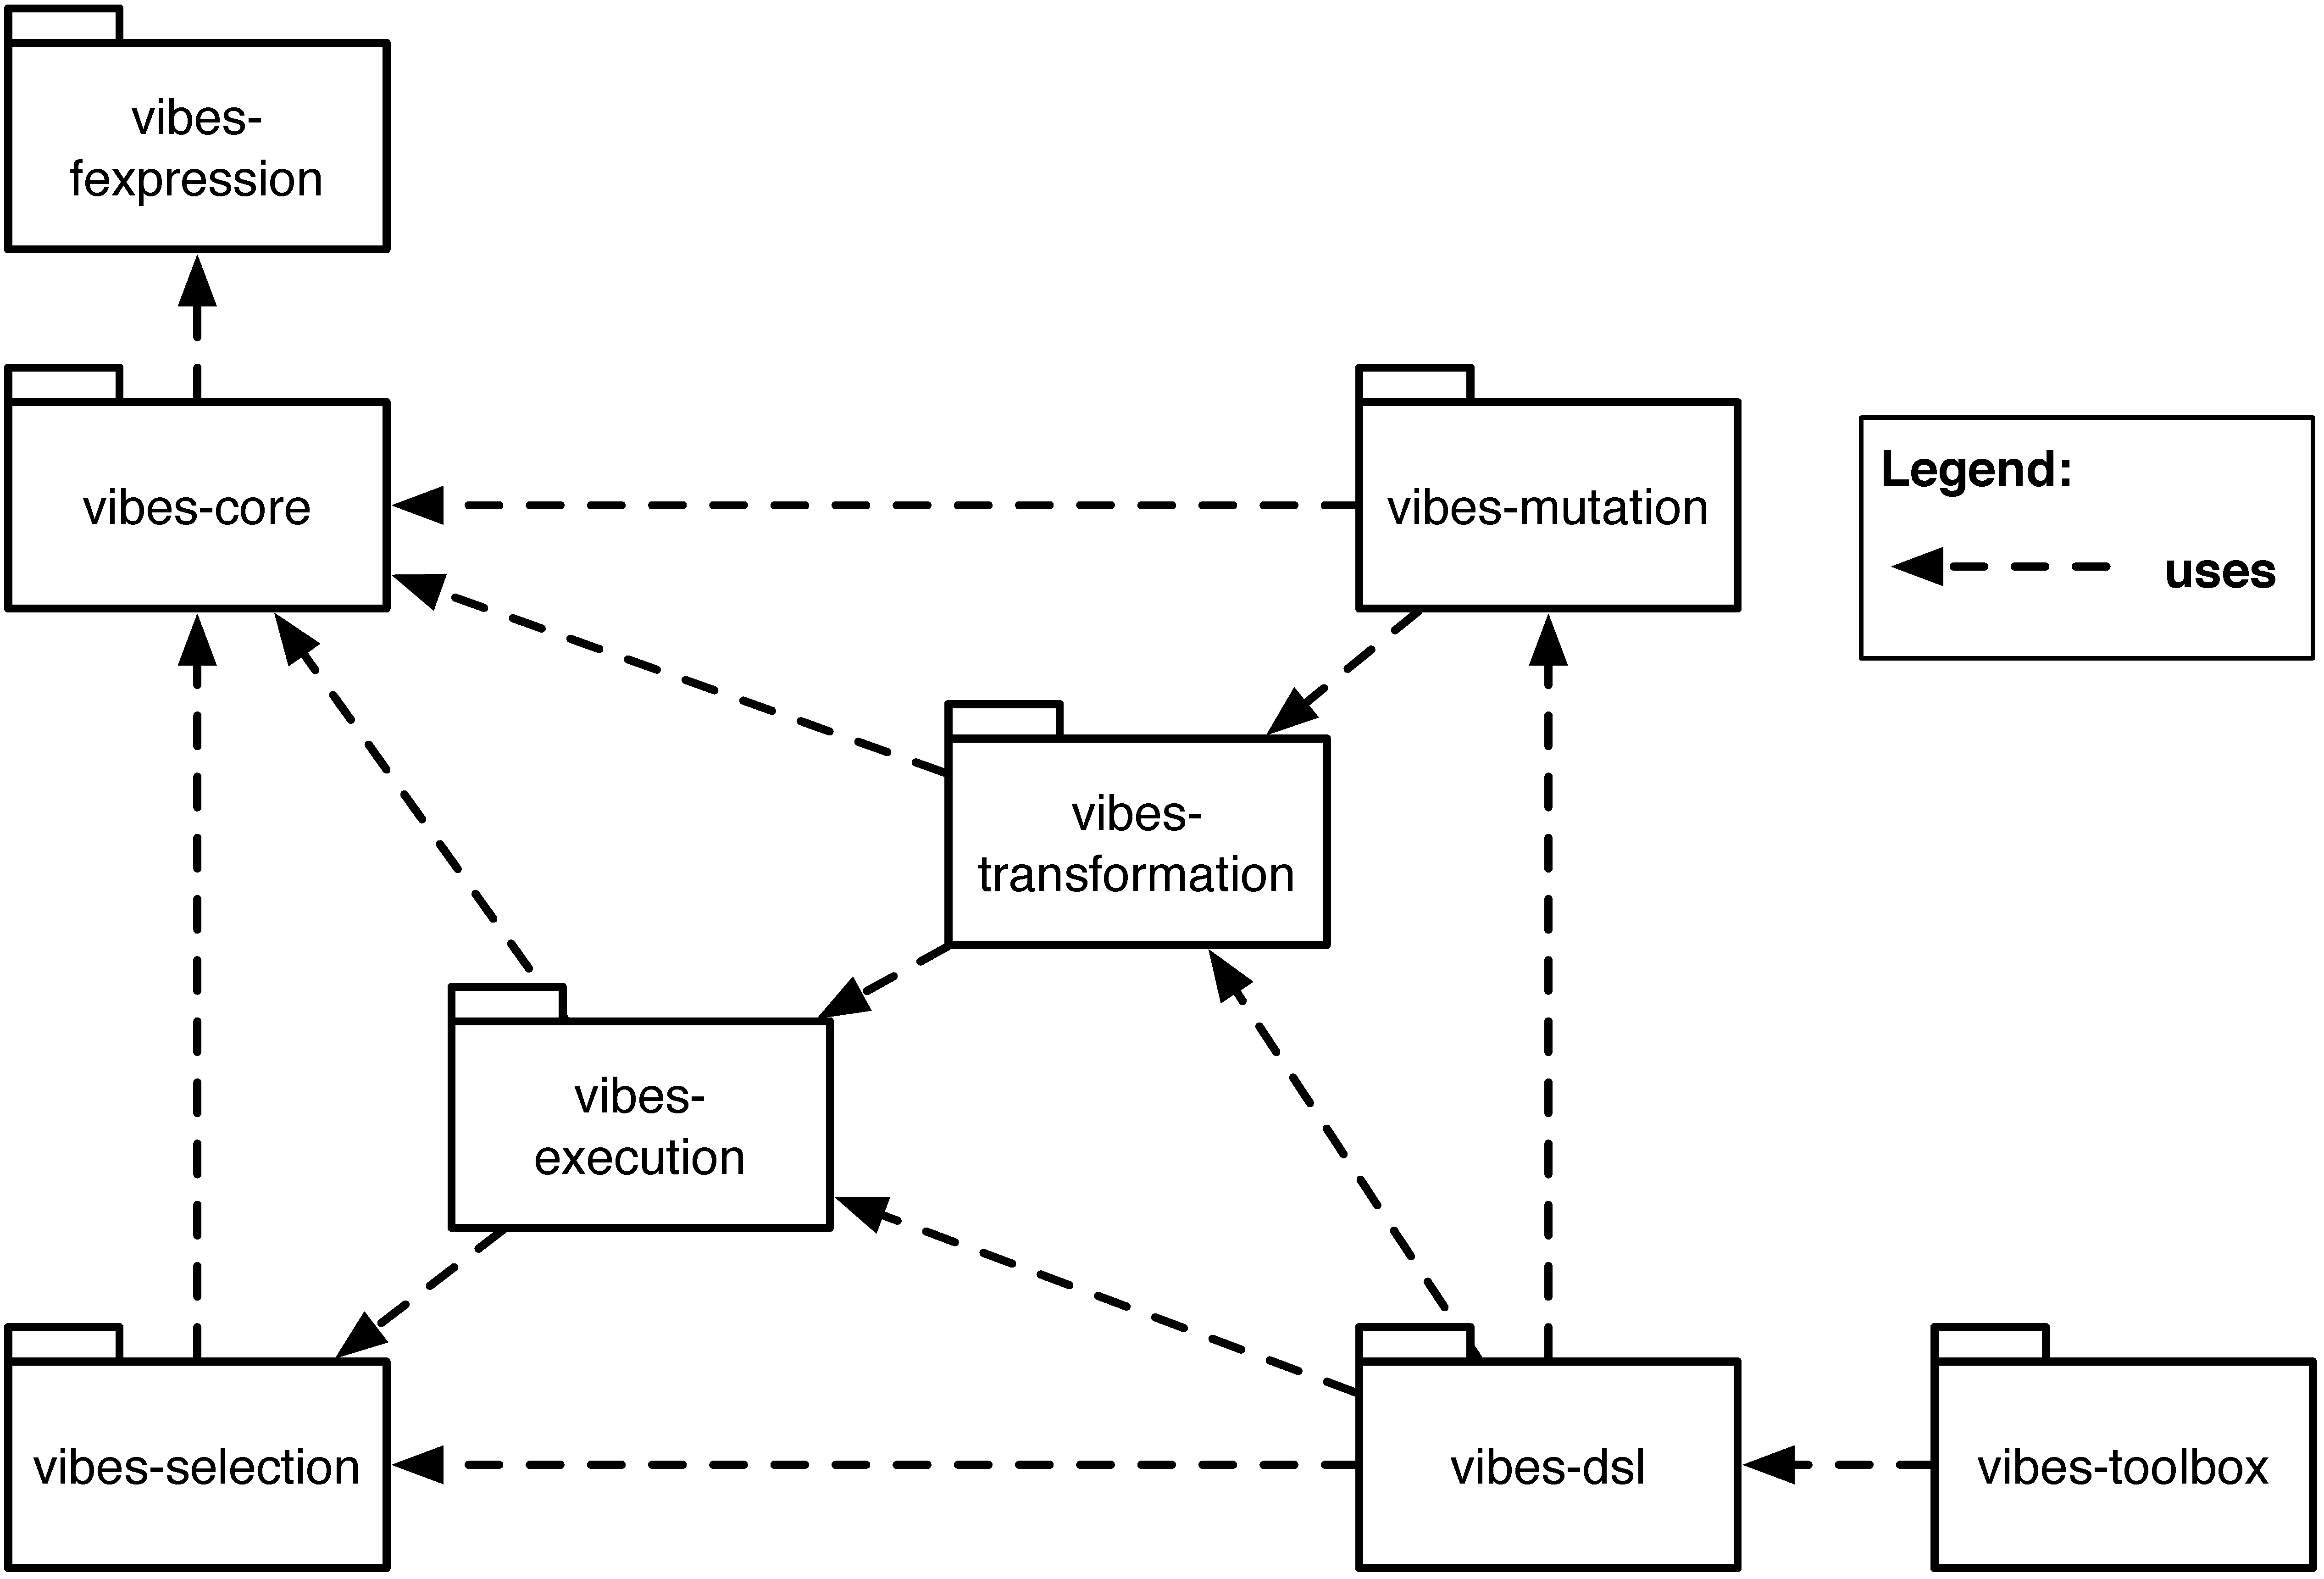
\includegraphics[width=110mm]{vibes-dependencies}
	\caption{\gls{VIBeS} modules dependency graph}
	\label{fig:vibesdependencies}
\end{figure} 

Maven allows to organise a project hierarchically. The root project is a \emph{Maven project}, while the sub-projects are \emph{Maven modules}. \gls{VIBeS}'s Maven project produces the artefact \texttt{be.unamur.info:vibes:1.1.6}, which is only a \gls{POM} without any associated Jar. \gls{VIBeS}'s project has several modules (with the same group identifier and version number as the parent project) regrouping different aspects of the framework. For instance, the modules \texttt{vibes-core} contains the core classes used to model \glspl{FTS}, module \texttt{vibes-selection} contains Java classes to perform test case selection from a \gls{FTS} model, \etc Figure \ref{fig:vibesdependencies} presents the different modules from \gls{VIBeS} and the dependencies between them: module \texttt{vibes-core} uses the \texttt{vibes-fexpression} modules that allows to represent and manipulate feature expressions; module \texttt{vibes-selection} presents an \gls{API} to select test cases from a transition system (\gls{FTS}, \gls{LTS}, or \gls{usage model}); module \texttt{vibes-execution} contains the \gls{API} to execute abstract test cases on the transition systems; \texttt{vibes-transformation} allows to transform, serialize, or deserialize the transition systems using different formalisms (\eg XML, DOT file, timbuk automata, \etc); module \texttt{vibes-mutation} contains the \gls{API} to perform mutation analysis; \texttt{vibes-dsl} encapsulates the different \gls{API} to present a unified Java DSL to perform the different testing activities using \gls{VIBeS}; and \texttt{vibes-toolbox} contains all the sub-modules that uses the Java DSL to implement toolboxes to perform particular tasks (\eg generate mutants). 

\begin{figure}
	\centering
	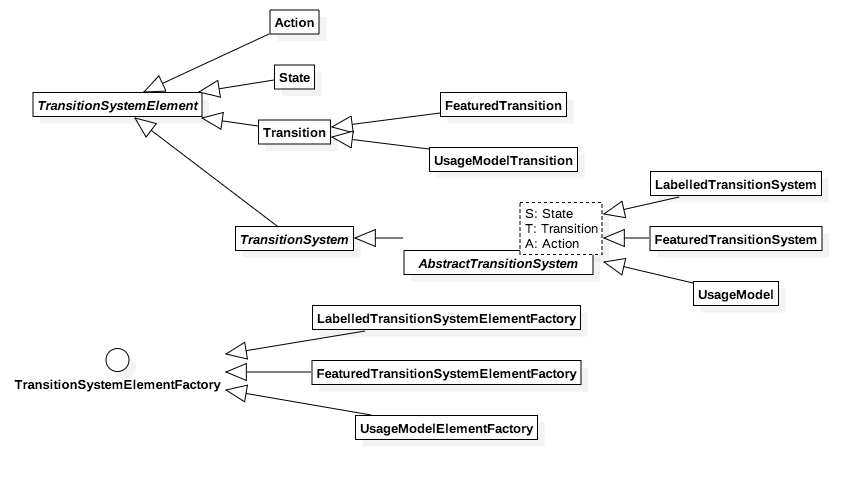
\includegraphics[width=\textwidth]{vibes-type-hierarchy}
	\caption{\gls{VIBeS} type hierarchy class diagram}
	\label{fig:vibestypehierarchy}
\end{figure} 

Classes from the \texttt{vibes-core} modules represent the transition systems used by \gls{VIBeS}. Figure \ref{fig:vibestypehierarchy} presents the class hierarchy of the different elements. Each element of a transitions system (actions, states, transitions, and the transition system itself) extends the \texttt{Tran\-si\-tion\-Sys\-tem\-Ele\-ment} class. Transitions are either simple transitions (\texttt{Transition} class) or transitions labelled by feature expression (\texttt{FeaturedTransition} class) or a probability (\texttt{UsageModelTransition} class). Transition systems (\texttt{Label\-led\-Tran\-sition\-System}, \texttt{Fea\-tu\-red\-Tran\-sit\-ion\-System}, and \texttt{Usage\-Mo\-del}) extends the \texttt{Ab\-stract\-Tran\-si\-tion\-System} class,  which is parametrized with the type of states, transitions, and actions used for this transition system (featured transitions for the \glspl{FTS} for instance). To manage the creation of the different elements of a transition system, a dedicated factory, extending \texttt{Tran\-si\-tion\-Sys\-tem\-Ele\-ment\-Facto\-ry}, is used.

Figure \ref{fig:vibescore} presents how transition systems are represented. A transition system (class \texttt{TransitionSystem}) is a collection of actions and states, with an initial state. Each state has incoming and outgoing transitions, and each transition is labelled with an action belonging to the same transition system. The default transition system implementation (class \texttt{AbstractTransitionSystem}) uses a factory to build the different states, actions, and transitions. This insures to respect the representation invariant of the class.

\begin{figure}
	\centering
	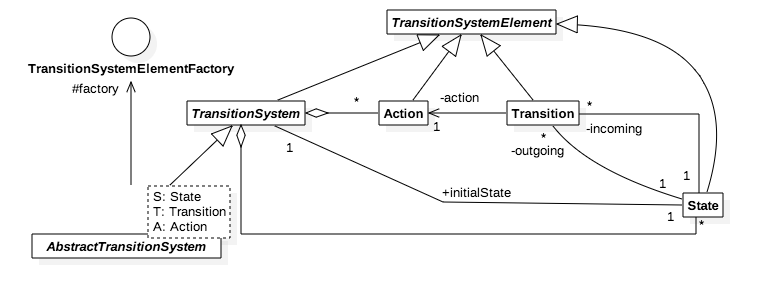
\includegraphics[width=\textwidth]{vibes-core}
	\caption{\gls{VIBeS} transition systems class diagram}
	\label{fig:vibescore}
\end{figure}


%%%%%%%%%%%%%%%%%%%%%%%%%%%%%%
\section{API usage}
%%%%%%%%%%%%%%%%%%%%%%%%%%%%%%

\label{sec:vibesusages}

The simplest way to use \gls{VIBeS} is to create a new Maven project and add a dependency to  \texttt{be.unamur.info:vibes-dsl:1.1.6}:
%
\begin{lstlisting}[language=XML,frame=single,numbers=none,morekeywords={dependency,groupId,artifactId,version}]
<dependency>
    <groupId>be.unamur.info</groupId>
    <artifactId>vibes-dsl</artifactId>
    <version>1.1.6</version>
</dependency>
\end{lstlisting}
This artefact contains an \gls{API} that encapsulates most of \gls{VIBeS} usages. The \texttt{vibes-dsl} module has been built following the same philosophy as the Apache Camel Java DSL\footnote{See \url{http://camel.apache.org}.} to chain method calls in order to facilitate the model definition, test case selection, mutation analysis, \etc

%------------------------------------
\subsection{Model definition}
%------------------------------------

Definition of a new \gls{FTS} is done by extending the \texttt{Featured\-Tran\-si\-tion\-Sys\-tem\-De\-fi\-ni\-tion} class  and implementing the abstract \texttt{define} method of that class. This method calls other inherited methods to define the initial state, states, actions, and transitions. For instance, the \gls{soda vending machine} \gls{FTS} from Section \ref{sec:casestudy:svm} is defined as:
%
\begin{lstlisting}[language=Java,frame=single,numbers=none]
public class SodaVendingMachineModel extends FeaturedTransitionSystemDefinition{
    
    private static final String[] S = new String[]{"s1", "s2", "s3", "s4", "s5", "s6", "s7", "s8", "s9"};

    @Override
    protected void define() {
        initial(S[0]); // Define the initial state

        from(S[0]).action("pay").fexpr("!f").to(S[1]);
        from(S[0]).action("free").fexpr("f").to(S[2]);
        
        from(S[1]).action("change").fexpr("!f").to(S[2]);
        from(S[2]).action("cancel").fexpr("c").to(S[3]);
        
        from(S[3]).action("return").fexpr("c").to(S[0]);
        from(S[3]).action("soda").fexpr("s").to(S[4]);
        from(S[3]).action("tea").fexpr("t").to(S[5]);
        
        from(S[4]).action("serveSoda").fexpr("s").to(S[6]);
        from(S[5]).action("serveTea").fexpr("t").to(S[6]);
        
        from(S[6]).action("take").fexpr("f").to(S[0]);
        from(S[6]).action("open").fexpr("!f").to(S[7]);
        
        from(S[7]).action("take").fexpr("!f").to(S[8]);
        from(S[8]).action("close").fexpr("!f").to(S[0]);
    }   
}
\end{lstlisting}
%
The model can be instantiated by calling the \texttt{getTransitionSystem} method:
%
\begin{lstlisting}[language=Java,frame=single,numbers=none]
FeaturedTransitionSystem svm = new SodaVendingMachineModel().getTransitionSystem();
\end{lstlisting}
%
Transitions may be tagged with an action or a feature expression. \Glspl{feature expression} must respect the following grammar:
%
\begin{lstlisting}[frame=single,numbers=none]
fexpression: 'true'
			| 'false'
			| featureName
			| '(' fexpression ')'
			| '!' fexpression
			| fexpression ('&&' | '||') fexpression ;

featureName: LETTER (LETTER | DIGIT)* ;

LETTER: 'A'..'Z' | 'a'..'z' | '_';
DIGIT: '0'..'9';
\end{lstlisting}
%
Feature names must begin by a letter, and may contain letters or digits. Operators have the following priority rules: negation ('\texttt{!}') takes precedence over conjunction ('\texttt{\&\&}') and disjunction ('\texttt{||}').

%------------------------------------
\subsection{Test suite selection}
%------------------------------------

Test suite selection may be done manually, or using one of the selection criterion defined in Chapter \ref{chap:coverage}. 

\paragraph{Manual test suite selection:}
%----------------------------------------

Manual selection is done by extending the \texttt{Test\-Set\-De\-fi\-ni\-tion} class. As for the model definition, the \texttt{define} method has to be implemented and call inherited methods to define the test cases:
%
\begin{lstlisting}[language=Java,frame=single,numbers=none]
public class ManualTestSuite extends TestSuiteDefinition{

    @Override
    protected void define() {
        id("testRefund").action("pay").action("change").action("cancel").action("return").end();
        id("testFreeTea").action("free", "tea", "serveTea", "take");
        id("testNoFreeSoda").action("pay", "change").action("soda", "serveSoda").action("open", "take", "close");
    }
}
\end{lstlisting}
%
Actions may be added one by one or by groups in the same \texttt{action} method call. The test suite is instantiated using the \texttt{getTestSet} method:
%
\begin{lstlisting}[language=Java,frame=single,numbers=none]
TestSet testSuite = new ManualTestSuite().getTestSet();
\end{lstlisting}
%


\paragraph{Random selection:}
%----------------------------------------

Random test suite selection selects a defined number of test cases by random walks in \gls{FTS}. This requires the \gls{feature model} of the \gls{FTS} from which test cases are selected to ensure that selected test cases are positive abstract test cases. This feature model is encapsulated in a constraint solver (Sat4j\footnote{See \url{http://www.sat4j.org}.} for instance), accessed trough a facade that implements the \texttt{SolverFacade} interface. To load the feature model, one may use a feature expression (a \gls{CNF} boolean expression representing the feature model) or load it from a DIMACS CNF file. In the following example, we load the feature model from a DIMACS CNF file:
%
\begin{lstlisting}[language=Java,frame=single,numbers=none]
// Feature model loading
DimacsModel featureModel = DimacsModel.createFromDimacsFile("svm.dimacs");
SolverFacade solver = new Sat4JSolverFacade(featureModel);  

// Random test suite selection
TestSet randomSuite = randomSelection(svm, solver);
\end{lstlisting}
%


\paragraph{All-states selection:}
%----------------------------------------

Selection of a test suite satisfying the all-state criterion is done by importing the \texttt{allStatesSelection} static method from the \texttt{AllStates} class:
%
\begin{lstlisting}[language=Java,frame=single,numbers=none]
// Feature model loading
DimacsModel featureModel = DimacsModel.createFromDimacsFile("svm.splot.dimacs");
SolverFacade solver = new Sat4JSolverFacade(featureModel);  

// All-states test suite selection
TestSet allStatesSuite = allStatesSelection(svm, solver);
\end{lstlisting}
%

\paragraph{Dissimilarity-driven selection:}
%----------------------------------------

Test suite selection using a dissimilarity heuristic is done using the \texttt{Dissimilar} class. The heuristic may be configured using the following methods:
%
\begin{lstlisting}[language=Java,frame=single,numbers=none]
// Feature model loading
DimacsModel featureModel = DimacsModel.createFromDimacsFile("svm.splot.dimacs");
SolverFacade solver = new Sat4JSolverFacade(featureModel);  

// Dissimilar selection
from(svm, solver)
	.during(30000) // specify duration
	// specify local or global distance and how to compute dissimilarity
	.withLocalMaxDistance(ftsDissimilarity(solver, levenshtein(), avg()))
	// Specify the number of test cases
	.generate(5);
\end{lstlisting}
%
Duration specifies how long the algorithm will run, using a local (\texttt{with\-Local\-Max\-Dis\-tance}) or global (\texttt{with\-Glo\-bal\-Max\-Dis\-tance}) distance computation. The distance itself is defined using one of the static methods that works on the actions alone (\texttt{hamming}, \texttt{jaccard}, \texttt{dice}, \texttt{antidice}, or \texttt{levenshtein}), or in combination with product distance (\texttt{fts\-Dis\-si\-mi\-la\-ri\-ty}), using a binary operator (\texttt{avg}, \texttt{mul}, or any other \texttt{Bi\-na\-ry\-Ope\-ra\-tor} object).

\paragraph{Usage-based selection:}
%----------------------------------------

Usage based selection is more complex. First, it requires to select a set of test cases in the \gls{usage model} using \texttt{Boun\-ded\-Pro\-ba\-bi\-li\-ty\-Ge\-ne\-ra\-tor} class. Those test cases are then executed on the \gls{FTS} that is pruned to keep only transitions activated by at least one test case. This is done using the \texttt{Prun\-ning.pru\-ne} method. Complete usage-based test suite selection is not yet encapsulated in \texttt{vibes-dsl}. This is part of our future work.

%-------------------------------------------------------
\subsection{Saving and loading models}
%-------------------------------------------------------

Models may be saved in XML format using the \texttt{Tran\-si\-tion\-Sy\-stem\-Xml\-Prin\-ter} class. To load a model from an XML file, one may use the \texttt{Tran\-si\-tion\-Sys\-tem\-Xml\-Loa\-ders} class:
%
\begin{lstlisting}[language=Java,frame=single,numbers=none]
// Load model
FeaturedTransitionSystem svm = loadFeaturedTransitionSystem("svm.xml");

// Save model
print(svm, "svm.xml");
\end{lstlisting}
%
The XML model of the soda vending machine is the following:
%
\begin{lstlisting}[language=XML,frame=single,numbers=none]
<?xml version="1.0" encoding="utf-8"?>
<fts xmlns="http://www.unamur.be/xml/fts/" xmlns:xsi="http://www.w3.org/2001/XMLSchema-instance">
  <start>state1</start>
  <states>
    <state id="state1">
      <transition action="pay" fexpression="!FreeDrinks" target="state2"/>
      <transition action="free" fexpression="FreeDrinks" target="state3"/>
    </state>
    <state id="state2">
      <transition action="change" fexpression="!FreeDrinks" target="state3"/>
    </state>
    ...
  </states>
</fts>
\end{lstlisting}

%-------------------------------------------------------
\subsection{Performing mutation analysis}
%-------------------------------------------------------

Mutation analysis consist of mutants generation (in an enumerative or \gls{FMM} approach) and mutants execution. Those analysis are done at the product level (on \glspl{LTS}), mutation analysis for \glspl{FTS} is part of our future works. 

\paragraph{Mutation operators configuration:}
%---------------------------------------------

Operators may be configured using the \texttt{Mu\-ta\-gen} class. This is useful to define the selection strategy of the elements to mutate. For instance, one can create a state missing (SMI) operator that will only remove particular states (chosen randomly):
%
\begin{lstlisting}[language=Java,frame=single,numbers=none]
MutationOperator op = Mutagen.stateMissing(svm)
	.stateSelectionStrategy(svm.getState("s4"), svm.getState("s8"), svm.getState("s9"))
	.done();
\end{lstlisting}
%
One may also configure a set of operators using an XML configuration file:
%
\begin{lstlisting}[language=XML,frame=single,numbers=none]
<?xml version="1.0" encoding="utf-8"?>
<config>
  <!-- Default mutant size (may be redefined) -->
  <mutantsSize>200</mutantsSize>
  <!-- Default selection strategies (may be redefined) -->
  <actionSelection>
    be.unamur.transitionsystem.test.mutation.RandomSelectionStrategy
  </actionSelection>
  <stateSelection>
    be.unamur.transitionsystem.test.mutation.RandomSelectionStrategy
  </stateSelection>
  <transitionSelection>
    be.unamur.transitionsystem.test.mutation.RandomSelectionStrategy
  </transitionSelection>
  <!-- Default uniqueness of each mutant (may be redefined) -->
  <unique>true</unique>
  <!-- Operators -->
  <operators>
    <operator>
      <class>be.unamur.transitionsystem.test.mutation.ActionExchange</class>
    </operator>
    ...
    <operator>
      <class>be.unamur.transitionsystem.test.mutation.WrongInitialState</class>
      <mutantsSize>100</mutantsSize>
      <actionSelection>be.dummy.MyActStrategy</actionSelection>
      <stateSelection>be.dummy.MyStStrategy</stateSelection>
      <transitionSelection>be.dummy.MyTrStrategy</transitionSelection>
      <unique>false</unique>
    </operator>
  </operators>
</config>
\end{lstlisting}
%
Default configuration (selection strategy, number of mutants to generate, uniqueness on mutant based on the selected operands of the operator) may be redefined for each mutation operator.

\paragraph{Mutants generation (enumerative approach):}
%-------------------------------------------------------

Mutants may be generated enumeratively: each mutant is generated in a new XML file. For instance:
%
\begin{lstlisting}[language=Java,frame=single,numbers=none]
LabelledTransitionSystem lts = loadLabelledTransitionSystem("product.xml");
configure("operatorsConfig.xml")
	.outputDir("mutants/") // Generates mutants in the given folder
	.mutate(lts);
\end{lstlisting}
%

\paragraph{Mutants generation (\gls{FMM} approach):}
%-------------------------------------------------------

One can also generate a \gls{FMM} and save it in an XML and a \gls{TVL} files :
%
\begin{lstlisting}[language=Java,frame=single,numbers=none]
LabelledTransitionSystem lts = loadLabelledTransitionSystem("product.xml");
FeaturedMutantsModel fmm = configure("operatorsConfig.xml")
	.ftsMutant("fmm.fts") // Generates FMM's FTS with given name
	.tvlMutant("fmm.tvl") // Generates FMM's FD in TVL format
	.mutate(lts);
\end{lstlisting}
%

\paragraph{Mutants execution:}
%------------------------------

Finally, execution of a test suite on the \gls{FMM} is done using the \texttt{get\-Alive\-Mu\-tants} static method of the \texttt{Fea\-tu\-red\-Mu\-tants\-Mo\-dels} class:
%
\begin{lstlisting}[language=Java,frame=single,numbers=none]
FExpression alive = getAliveMutants(testSuite.get(0), fmm);
solver.addConstraint(alive);
Iterator<Configuration> solutions = solver.getSolutions();
while(solutions.hasNext()) {
	System.out.println(solutions.next());
}
\end{lstlisting}
%

%------------------------------------
\subsection{\gls{VIBeS} toolboxes}
%------------------------------------

\gls{VIBeS} architecture in Maven modules allows to do rapid prototyping. Module \texttt{vibes-dsl} encapsulates the common operations performed during the testing activities to reduce as much as possible custom developments. Beside \texttt{vibes-dsl} module,  \gls{VIBeS} also comes with a set of toolboxes. Each of those toolbox is a executable Jar file with a command line interface that may be used to perform standard tasks. The existing toolboxes are:
\begin{itemize}
\item \texttt{toolbox-model-statistics}: to print statistics about a transition system;
\item \texttt{toolbox-testcase-generation}: to select test suites using various criteria;
\item \texttt{toolbox-transformation}: to transform an XML transition system to other formats (\eg Graphviz DOT);
\item \texttt{toolbox-products-analyze}: to print the number of products for a given feature model and a given feature expression;
\item \texttt{toolbox-mutant-generation}: to generate mutants (enumeratively or using a \gls{FMM});
\item \texttt{toolbox-fmm-execution}: to execute test cases on a \gls{FMM};
\item \texttt{toolbox-mutation-equivalence}: to detect equivalent mutants using simulation or automata language equivalence;
\item \texttt{toolbox-mutant-sampling}: to sample a set of mutants (from different orders) from a given \gls{FMM}.
\end{itemize}


%%%%%%%%%%%%%%%%%%%%%%%%%%%%%%%%%%%%
\section{Wrap up}
%%%%%%%%%%%%%%%%%%%%%%%%%%%%%%%%%%%%

\label{sec:vibesperspectives}

In this chapter, we present \gls{VIBeS}, the implementation of our testing framework. We use \gls{VIBeS} to perform various testing activities, including model definition, test suite selection, and mutation analysis. 

\gls{VIBeS} is built as a Maven project with several modules. Each module is dedicated to one particular aspect of the testing activities. Test engineers may use \gls{VIBeS} by accessing the API of the different modules, or by using the Java DSL that encapsulates API calls and simplifies usages. 

This modular architecture allows to perform rapid prototyping while allowing adhoc developments for specific needs. We choose to use Java as the interface language for the test engineer rather than a dedicated DSL or modelling language. This avoids to switch between syntaxes and, we assume, lowers the learning curve for new users. This idea stems from industrial practices (like Apache Camel\footnote{See \url{http://camel.apache.org}.}) and seems to be confirmed by other trending behavioural testing tools (like Cucumber \cite{cucumber} where, except for the behavioural description of the system, all elements are defined in Java).

%Future work includes a refactoring and refinement of \gls{VIBeS} Java DSL to standardize names and encapsulate calls to the most recent parts of the API (like mutant equivalence detection and usage-based test suite selection). Finally, performance of the different test suite selection algorithms and mutant execution algorithms may be improved in order to reduce execution time and memory consumption.

